\documentclass[11pt,letterpaper]{article}
\usepackage[lmargin=1in,rmargin=1in,tmargin=1in,bmargin=1in]{geometry}
\usepackage{../style/homework}
\usepackage{../style/commands}
\setbool{quotetype}{true} % True: Side; False: Under
\setbool{hideans}{true} % Student: True; Instructor: False

% -------------------
% Content
% -------------------
\begin{document}

\homework{20: Due 12/15}{The origins of graph theory are humble, even frivolous.}{Norman Biggs}

% Problem 1
\problem{10} Consider the graphs $G$ and $H$ given below. 
	\[
	\begin{tikzpicture}
        \begin{scope}[very thick, decoration= {markings, mark=at position 0.5 with {\arrow{>}}}] 
        
	% Undirected
	\draw[line width=0.05cm, bend left= 30] (-1,1) to (1,1);
	\draw[line width=0.05cm, bend right= 30] (-1,1) to (1,1);
	\draw[line width=0.05cm] (-1,1) to (0,0);
	\draw[line width=0.05cm] (1,1) to (0,0);
	\draw[line width=0.05cm, bend right= 30] (-1,1) to (0,-1);
	\draw[line width=0.05cm, bend left= 30] (1,1) to (0,-1);
	\draw[line width=0.05cm] (0,0) to (0,-1);
	\draw[line width=0.05cm] (0,-1) to (0,-2);
	\draw[line width=0.05cm] (0,-2.3) circle (0.3);
	
	\draw[fill= black] (0,0) circle (0.1);
	\draw[fill= black] (-1,1) circle (0.1);
	\draw[fill= black] (1,1) circle (0.1);
	\draw[fill= black] (0,-1) circle (0.1);
	\draw[fill= black] (0,-2) circle (0.1);
	
	\node at (-1.4,1) {$v_0$};
	\node at (1.4,1) {$v_1$};
	\node at (-0.25,-0.2) {$v_2$};
	\node at (-0.3,-1.1) {$v_3$};
	\node at (-0.25,-1.75) {$v_4$};
	
	\node at (0,1.5) {$e_1$};
	\node at (0,0.9) {$e_2$};
	\node at (-0.9,-0.4) {$e_3$};
	\node at (-0.63,0.35) {$e_4$};
	\node at (0.65,0.35) {$e_5$};
	\node at (0.9,-0.4) {$e_6$};
	\node at (0.25,-1.5) {$e_7$};
	\node at (0.4,-2.7) {$e_8$};
	
	\node at (0,-3.5) {$G$};
	
	% Directed
	\tikzset{shift={(7,-1.2)}}
	\draw[line width= 0.05cm, postaction={decorate}] (-1,1.732) to (1,1.732);
	\draw[line width= 0.05cm, postaction={decorate},bend right= 80] (1,1.732) to (-1,1.732);
	\draw[line width= 0.05cm, postaction={decorate}] (0,0) to (-1,1.732);
	\draw[line width= 0.05cm, postaction={decorate}] (0,0) to (1,1.732);
	\draw[line width=0.05cm, postaction={decorate}] (-1,1.732) arc (0:-360:0.5);
	\draw[line width=0.05cm, postaction={decorate}] (1,1.732) arc (180:540:0.5);
	\draw[line width=0.05cm, postaction={decorate}] (0,0) arc (90:-270:0.5);
	
	
	\draw[fill= black] (-1,1.732) circle (0.1);	
	\draw[fill= black] (0,0) circle (0.1);
	\draw[fill= black] (1,1.732) circle (0.1);
	
	\node at (-0.95,2.3) {$w_1$};
	\node at (0.95,2.3) {$w_2$};
	\node at (0.4,0.1) {$w_3$};
	
	
	\node at (-2.3,1.732) {$f_1$};
	\node at (0,2.65) {$f_2$};
	\node at (0,1.40) {$f_3$};
	\node at (-0.75,0.7) {$f_4$};
	\node at (0.75,0.7) {$f_5$};
	\node at (0,-1.3) {$f_6$};
	\node at (2.4,1.732) {$f_7$};
	
	\node at (0,-2.3) {$H$};
	\end{scope}
	\end{tikzpicture}
	\]

\begin{enumerate}[(a)]
\item Find $\deg v_2$, $\deg v_4$, and $\deg G$.
\item Is $G$ connected? Explain. Is $G$ simple? Explain.
\item Find $\deg^+ \!w_1$ and $\deg^- \!w_1$ as well as $\deg^+ \!w_2$ and $\deg^- \!w_2$. 
\item Find a trail in $H$ that is not a path. 
\item Does $H$ have any sources or sinks? Explain. 
\end{enumerate}



\newpage



% Problem 2
\problem{10} Suppose you have two graphs, $G$ and $H$, where $G$ is undirected and $H$ may be undirected or directed. The adjacency matrices of $G$ and $H$ are given below. \par
	\def\matrixG{%
	\begin{matrix}
	0 & 1 & 1 & 0 \\
	1 & 1 & 0 & 1 \\
	1 & 0 & 0 & 2 \\
	0 & 1 & 2 & 0 
	\end{matrix}
	}%
	\def\matrixH{%
	\begin{matrix}
	0 & 0 & 1 & 0 & 0 \\
	1 & 0 & 0 & 0 & 0 \\
	0 & 1 & 0 & 0 & 0 \\
	0 & 0 & 0 & 2 & 0 
	\end{matrix}
	}%
	\[
	\left(\vphantom{\matrixG} \right.\kern-2\nulldelimiterspace
  \underbrace{\matrixG}_{G} \kern-\nulldelimiterspace\left.\vphantom{\matrixG} \right) \qquad
  	\left(\vphantom{\matrixH} \right.\kern-2\nulldelimiterspace
  \underbrace{\matrixH}_{H} \kern-\nulldelimiterspace\left.\vphantom{\matrixH} \right)
	\]

\begin{enumerate}[(a)]
\item Draw the graph of $G$.
\item Does $G$ have a loop? Justify your answer using \textit{only} the adjacency matrix of $G$.
\item Draw the graph of $H$.
\item Is $H$ undirected or directed? Justify your answer using \textit{only} the adjacency matrix of $H$.
\item Do $G$ or $H$ have multiple edges? Explain your answer using only the adjacency matrix of $G$ and $H$, respectively. 
\end{enumerate}



\newpage



% Problem 3
\problem{10} Showing all your work and fully justifying your responses, complete the following:
	\begin{enumerate}[(a)]
	\item Draw the graph of $K_5$. How many vertices and edges does $K_5$ have? For $n \geq 1$, what are $|V(K_n)|$ and $|E(K_n)|$?
	\item Draw the graph of $K_{3, 5}$. How many vertices and edges does $K_{3, 5}$ have? For $m, n \geq 1$, what are $|V(K_{m, n})|$ and $|E(K_{m, n})|$?
	\item If $G$ is a simple graph, the complement of $G$, denoted $\widetilde{G}$, is a graph with $V(G)= V(\widetilde{G})$ and two vertices are adjacent in $\widetilde{G}$ if and only if they are not adjacent in $G$. Find the complement of the graph given below. Is $G$ connected? Is $\widetilde{G}$ connected? 
		\[
		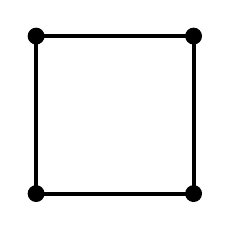
\begin{tikzpicture}[scale=2]
		\draw[line width= 0.05cm] (0,0) -- (1,0) -- (1,1) -- (0,1) -- (0,0);
		
		\draw[fill=black] (0,0) circle (0.05); 
		\draw[fill=black] (1,0) circle (0.05); 
		\draw[fill=black] (1,1) circle (0.05); 
		\draw[fill=black] (0,1) circle (0.05); 
		\end{tikzpicture}
		\]
	\end{enumerate}



\newpage



% Problem 4
\problem{10} Below are three graphs: $G_1$, $G_2$, and $G_3$. Determine which, if any, of the graphs are isomorphic. If two given graphs are isomorphic, show that they are isomorphic. If two graphs are not isomorphic, give at least two reasons why they are not isomorphic. 
	\[
	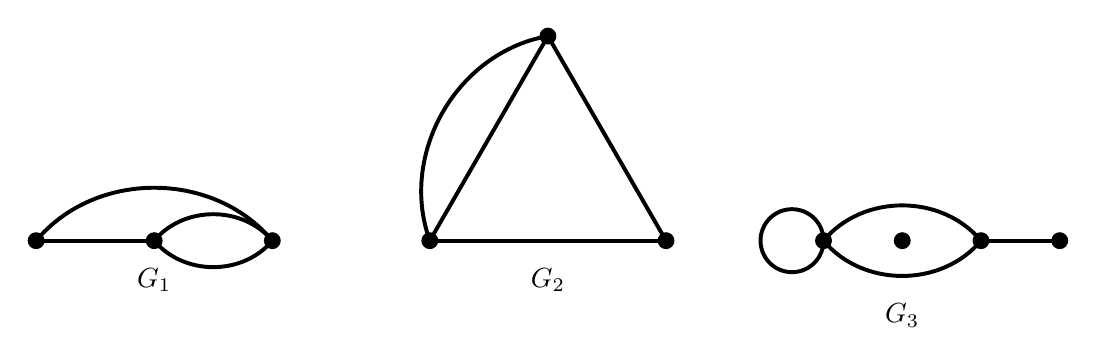
\begin{tikzpicture}
	% Graph 1
	\draw[line width=0.05cm] (0,0) -- (1.5,0);
	\draw[line width=0.05cm, bend left= 50] (1.5,0) to (3,0);
	\draw[line width=0.05cm, bend right= 50] (1.5,0) to (3,0);
	\draw[line width=0.05cm, bend left= 50] (0,0) to (3,0);

	\draw[fill=black] (0,0) circle (0.1); 
	\draw[fill=black] (1.5,0) circle (0.1); 
	\draw[fill=black] (3,0) circle (0.1); 
	
	\node at (1.5, -0.5) {$G_1$}; 
	
	% Graph 2
	\tikzset{shift={(5,0)}}
	
	\draw[line width=0.05cm] (0,0) to (1.5,2.598);
	\draw[line width=0.05cm, bend left= 50] (0,0) to (1.5,2.598);
	\draw[line width=0.05cm] (1.5,2.598) to (3,0);
	\draw[line width=0.05cm] (0,0) to (3,0);

	\draw[fill=black] (0,0) circle (0.1); 
	\draw[fill=black] (1.5,2.598) circle (0.1); 
	\draw[fill=black] (3,0) circle (0.1); 
	
	\node at (1.5,-0.5) {$G_2$};
	
	% Graph 3
	\tikzset{shift={(5,0)}}
	
	\draw[line width=0.05cm] (-0.4,0) circle (0.4);
	\draw[line width=0.05cm, bend left= 50] (0,0) to (2,0);
	\draw[line width=0.05cm, bend right= 50] (0,0) to (2,0);
	\draw[line width=0.05cm] (2,0) to (3,0);
		
	\draw[fill=black] (0,0) circle (0.1);
	\draw[fill=black] (1,0) circle (0.1);
	\draw[fill=black] (2,0) circle (0.1);
	\draw[fill=black] (3,0) circle (0.1);
	
	\node at (1.0,-0.95) {$G_3$};
	\end{tikzpicture}
	\]

% determine definitions
% draw from adjacency
% draw K5, K3, 5 & complement
% Determine iso???









\end{document}